\documentclass[12pt]{article}
\usepackage{mathtools}
\addtolength{\textheight}{.5in}
\addtolength{\textwidth}{1in}
\addtolength{\topmargin}{-.25in}
\addtolength{\evensidemargin}{-.5in}
\addtolength{\oddsidemargin}{-.5in}
\usepackage{listings}
\lstset{
  basicstyle=\small\ttfamily,
  frame=lrtb,
  showstringspaces=false,
}
\begin{document}

\section{Problem 1}
a) The number of stars, $n$, is given by integrating the Salpeter function over the mass range

$$ n = \frac{1}{M_{\odot}} \int^{M_{u}}_{M_{l}} \xi_{0} (M/M_{\odot})^{-2.35} \mathrm{d}M $$

$$ n = \frac{\xi_{0}}{1.35} [(M_{l}/M_{\odot})^{-1.35} - (M_{u}/M_{\odot})^{-1.35}] \approx \frac{\xi_{0}}{1.35} (M_{l}/M_{\odot})^{-1.35} $$

since the number goes as a power law with a negative power, and $M_{l}$ is much smaller than $M_{u}$, the first term in the difference dominates, and the number of stars is sensitive to the lower limit on the mass

b) The stellar mass can be obtained by weighting the salpeter function by stellar mass

$$ M = \frac{1}{M_{\odot}} \int^{M_{u}}_{M_{l}} M/M_{\odot} \xi_{0} (M/M_{\odot})^{-2.35} \mathrm{d}M = \frac{1}{M_{\odot}} \int^{M_{u}}_{M_{l}} \xi_{0} (M/M_{\odot})^{-1.35} \mathrm{d}M $$

$$ M = \frac{\xi_{0}}{0.35} [(M_{l}/M_{\odot})^{-.35} - (M_{u}/M_{\odot})^{-.35}]  \approx \frac{\xi_{0}}{0.35} (M_{l}/M_{\odot})^{-.35}$$

Since each the number and mass go as a power law with a negative power, and $M_{l}$ is much smaller than $M_{u}$, the first term in the difference dominates, and the number of stars is sensitive to the lower limit on the mass

c) Simmilarly, the luminosity is obtained by weighting the mass function by the Luminosity-Mass relation

$$ L = \frac{L_{\odot}}{M_{\odot}} \int^{M_{u}}_{M_{l}} (M/M_{\odot})^{3.5} \xi_{0} (M/M_{\odot})^{-1.35} \mathrm{d}M = \frac{L_{\odot}}{M_{\odot}} \int^{M_{u}}_{M_{l}} \xi_{0} (M/M_{\odot})^{2.15} \mathrm{d}M $$

$$ L = \frac{\xi_{0} L_{\odot}}{3.15} [(M_{u}/M_{\odot})^{3.15} - (M_{l}/M_{\odot})^{3.15}] \approx  \frac{\xi_{0} L_{\odot}}{3.15} (M_{u}/M_{\odot})^{3.15}$$

For luminosity, the function goes as a powerlaw with positive power, $[(M_{u}/M_{\odot})^{3.15} - (M_{l}/M_{\odot})^{3.15}]$. And since $M_{l}$ is much smaller than $M_{u}$, the upper mass term will dominate in the differences. Thus, luminosity is more sensitive to the upper limit on the mass

Using these results we can evaluate the fraction of stars for a mass range $M_{l} = .3M_{\odot}$ up to $5M_{\odot}$-which excludes the upper limit

$$ [.3^{-1.35} - 5^{-1.35}] / [.3^{-1.35} - M_{u}^{-1.35}] \approx [.3^{-1.35} - 5^{-1.35}] / [(.3)^{-1.35}] = .978 $$

This means the stars in the excluded range, $5M_{\odot} - M_{u}$ account for 2.2 percent of the stars. Doing this exercise over for the mass gives us

$$ [.3^{-.35} - 5^{-.35}] / [.3^{-.35} - M_{u}^{-.35}] \approx [.3^{-.35} - 5^{-.35}] / [(.3)^{-.35}] = .626 $$

This means the stars in the excluded range, $5M_{\odot} - M_{u}$ account for about 37 percent of the mass

d) If the pleiades has a total mass of 800 solar masses, using our result from b and keeping the lower limit .3 solar masses

$$ 800 \, M_{\odot} = \frac{\xi_{0}}{0.35} (.3)^{-.35}, \xi_{0} = 800 \, M_{\odot} \,0.35(.3)^{.35} \approx 187.7 $$

$$ \frac{187.7}{1.35} (.3)^{-1.35} = 703$$

we get about 700 stars, as expected. To compute the luminosity the heavy stars contribute,

$$[10^{3.15} - 5^{3.15}] / 10^{3.15} \approx .89 $$

These heavy stars account for about 89 percent of the total luminosity

The Pleadies cluster has a population of stars with masses greater than 5 solar masses, from looking at the Salpeter plot. This means the luminosity will be dominated by the heaviest few stars, who will outshine the other members. On the other hand, globular clusters are old. Their heavy O and B stars have died long ago, so we are only left with the stars with masses less than 5 solar masses, which all have similar luminosities.

\section{Problem 2}

$m$ = -2.5 Log($f$) + $ZP$ or using the laws of logs

$$ m = \frac{-2.5 Ln(Rf}{Ln(10)} + ZP $$

If ZP is well known and has no error, then the uncertainty in $m$ is given by

$$\sigma_{m} = |\frac{\partial m}{\partial R}  \sigma_{R}| = \frac{2.5}{Ln(10)f}  \sigma_{f} = \frac{2.5}{Ln(10)} \frac{\sigma_{f}}{f}$$

If the uncertainty in $m$ is .3, then the fractional error in the flux is also about .3. This is because


$$ \frac{2.5}{Log(10)} \approx 1 $$

\begin{lstlisting}[language=Python][frame=single]
import numpy as np

#generate distances, and absolute magnitudes.
#use to calculate apparent mags
dist = np.random.uniform(low=70, high=130, size=2000)
m_abs=np.random.normal(loc=4.83, scale=.3, size=2000)
m_apa=5*np.log10(dist) - 5 + m_abs

#make a mask to show only elements
#that are brighter than aparent mag 10
bright_mask = m_apa < 10
print 'the fraction of stars seen is %.3f'
	 %(float(m_apa[bright_mask].size) / m_apa.size)
print 'the mean absolute magnitude of observed stars is %.3f Mags'
	 % (m_abs[bright_mask].mean())
\end{lstlisting}

gives the following output
\begin{lstlisting}[frame=none]
the fraction of stars seen is 0.635
the mean absolute magnitude of observed stars is 4.711 Mags
\end{lstlisting}
These stars are slightly brighter. However, the mean absolute magnitude of the sample falls within 1 sigma of the mean of the sky's stars,ianso this difference is well explained by the variance.
\begin{lstlisting}
print "the average distance of our sample is %.3f pc" % 
	(dist[bright_mask].mean())
\end{lstlisting}

\begin{lstlisting}[frame=none]
the average distance of our sample is 90.643 pc
\end{lstlisting}
our sample is biased towards stars that are closer, which is to be expected since they appear brighter by virtue of being closer. The mean distance for the entire sky we created is about 100 pc. 

making assumptions about our observed stars
\begin{lstlisting}
sample_dist = 10**((m_apa[bright_mask] - 4.83 + 5)/5.0)
print "the average calculated distance of the sample is %.3f pc" 
	%(sample_dist.mean())
\end{lstlisting}
\begin{lstlisting}[frame=none]
the average calculated distance of the sample is 87.490 pc
\end{lstlisting}

our new distances are biased inward still. This is because we started off with a systematically infected sample of observed stars. Additionally, the mean absolute magnitude we used was for a sample of stars is a bit too faint. To wind up with the reported apparent magnitudes, we would have to scoot our sample stars in a bit closer.

\begin{lstlisting}
z_metal = np.random.normal(loc=.6, scale=.1, size=2000)
z_mag_cor = -.87*np.log10(z_metal)
m_ap_met = m_apa + z_mag_cor
samp_b_mask = [(m_ap_met < 10) & (dist > 90) 
	& (dist < 110) & (z_metal > 0.0)]
samp_c_mask = [(m_ap_met < 10) 
	& (dist > 110) & (z_metal > 0.0)]

print "the average metalicity of sample stars observed in region b
	 is %.3f" % (z_metal[samp_b_mask].mean())
print "the average metalicity of sample stars observed in region c 
	is %.3f" % (z_metal[samp_c_mask].mean())
\end{lstlisting}

\begin{lstlisting}[frame=none]
the average metalicity of sample stars observed in region b is 0.614
the average metalicity of sample stars observed in region c is 0.635
\end{lstlisting}
The stars are increasingly metal rich. This is because lower metallicity stars have greater extinction, and are less likely to be observed in our sample. The greater distance in region b and c compounds this effect, favoring more metal rich stars the further away you look.
\section{Problem 3}

Use Poisson's equation for gravity
$$\nabla^{2} \phi = 4\pi G \rho $$
$$\nabla^{2} \phi = -\frac{1}{r^{2}} \frac{\partial}{\partial r} (r^2 \frac{\partial }{\partial r} ) \sigma^{2} \ln (1 + r/a_{N} ) (r/a_{N})^{-1}$$
$$\nabla^{2} \phi = -\frac{1}{r^{2}} \frac{\partial}{\partial r} \sigma^{2}[ (1 + r/a_{N})^{-1}r-a_{N} \ln (1 + r/a_{N})]$$
$$\nabla^{2} \phi = -\frac{1}{r^{2}}  \sigma^{2}[ (1 + r/a_{N})^{-1} -  (1 + r/a_{N})^{-2} r/a_{N} -  (1 + r/a_{N})^{-1}]$$
$$\nabla^{2} \phi =  \sigma^{2}  (1 + r/a_{N})^{-2} (ra_{N})^{-1} $$

now $\sigma^{2}_{N} = 4\pi G \rho_{N} a_{N}^2$

$$\nabla^{2} \phi =   4\pi G \rho_{N} (1 + r/a_{N})^{-2} (r/a_{N})^{-1} $$

from which we can pick off $\rho_{NFW}(r) = \frac{\rho_{N}}{(r/a_{N})(1 + r/a_{N})^{2}}$

Now circular motions have accelerations $\mathbf{a} = V^{2}/r$. We can obtain the acceleration from the potential using $-\nabla \phi = \mathbf{a}$. The acceleration is inward, in the negative radial direction.
$$ V^{2} = r \nabla \phi = \frac{\partial}{\partial r}  \sigma^{2} \ln (1 + r/a_{N} ) (r/a_{N})^{-1} = r\sigma^{2}[\ln (1 + r/a_{N})a_{N}(r)^{-2} - (1 + r/a_{N})^{-1}/r] $$
$$ V^{2}  = \sigma^{2} [\frac{\ln(1 + r/a_{N})}{r/a_{N}} - \frac{1}{1 + r/a_{N}}] $$

\section{Problem 4}
The observed radial velocity is the difference of the sun's velocity and the satellite's velocity along the line of sight. To project the suns  circular velocity to the satellite's azimuth angle, first introduce a factor of cos(b). Now to get the projection along the line of sight (along 'd' in the provided figure) we have to introduce a factor of sin(l). So putting this all together, we have $V_{\odot} = V - V_{0}\sin(l)\cos(b), V = V_{\odot} + V_{0}\sin(l)\cos(b)$

Using the Virial theorem, the mean KE is -.5 the mean PE.

$$ r V^{2} / G = M_{MW}  $$

\begin{lstlisting}[language=Python]
from astropy import units as u
from astropy import constants as c
d=np.array([49, 58, 120,25, 270, 72,
	207, 83, 100, 64, 72]) * u.kiloparsec 
Vr=np.array([274, 148, 53, 170, 285,
             107, 76, 225, 223, -247,
             -293]) *u.kilometer / u.second 
l=np.array([280, 303, 237, 6, 226,228,
            220, 244, 260, 105, 86]) * u.degree
b=np.array([-33, -44, -66, -14, 49,
            -83, 67, 42, -22, 45, 35]) * u.degree
gal_names=['Large MC', 'Small MC', 'Fornax', 'Sagittarius',
       'Leo I', 'Sculptor', 'Leo II', 'Sextans', 'Carina',
       'Ursa Minor','Draco']
Vsun= 220*u.kilometer/u.second

mass= d * np.square((Vr +Vsun *np.cos(b.to(u.radian))*
                     np.sin(l.to(u.radian))))/c.G

\end{lstlisting}

The table below shows the calculated solar masses. The mean mass is $2.7e11 \odot $, which is an order of magnitude short. I checked and rechecked, but I can't figure out what I did wrong.

\begin{table}
\begin{tabular}{cccccc}
Galaxy & d & Vr & l & b & Calc MW Mass \\
 & $\mathrm{kpc}$ & $\mathrm{km\,s^{-1}}$ & $\mathrm{{}^{\circ}}$ & $\mathrm{{}^{\circ}}$ & $\mathrm{M_{\odot}}$ \\
Large MC & 49.0 & 274.0 & 280.0 & -33.0 & 97023251699.3 \\
Small MC & 58.0 & 148.0 & 303.0 & -44.0 & 3146210844.87 \\
Fornax & 120.0 & 53.0 & 237.0 & -66.0 & 13556820927.3 \\
Sagittarius & 25.0 & 170.0 & 6.0 & -14.0 & 214919697306.0 \\
Leo I & 270.0 & 285.0 & 226.0 & 49.0 & 2.06006546934e+12 \\
Sculptor & 72.0 & 107.0 & 228.0 & -83.0 & 126894013234.0 \\
Leo II & 207.0 & 76.0 & 220.0 & 67.0 & 20707775160.0 \\
Sextans & 83.0 & 225.0 & 244.0 & 42.0 & 117541706101.0 \\
Carina & 100.0 & 223.0 & 260.0 & -22.0 & 11371779575.5 \\
Ursa Minor & 64.0 & -247.0 & 105.0 & 45.0 & 139214729236.0 \\
Draco & 72.0 & -293.0 & 86.0 & 35.0 & 214555397212.0 \\
\end{tabular}
\caption{calculated mass of the milky way using satellite galaxies}
\end{table}
\section{Problem 5}
\begin{lstlisting}[language=Python]
#import helpful things and read data
from astropy.io import ascii
from astropy.table import Table
hip = ascii.read('hip_main.dat', delimiter='|')

#grab the columns we need
#give them meaningful names
hip_sub = hip[['col6', 'col12','col17','col38','col39']]
hip_sub.rename_column('col6', 'mV')
hip_sub.rename_column('col12','paralax')
hip_sub.rename_column('col17','paralax_err')
hip_sub.rename_column('col38','B-V')
hip_sub.rename_column('col39','B-V_err')

#mask out data with fractional errors that are too big
tab_mask = (hip_sub['B-V_err'] < 0.03) & 
	(hip_sub['paralax_err']/hip_sub['paralax'] <= 0.1 )
clean_hip = hip_sub[tab_mask].filled([np.nan])

#calculate distances and absolute Mags
clean_hip['dist'] = 1./(1e-3 *clean_hip['paralax'])
clean_hip['MV'] = clean_hip['mV'] + 5 
	- 5*np.log10(clean_hip['dist'])
\end{lstlisting}

\begin{figure}
\centering
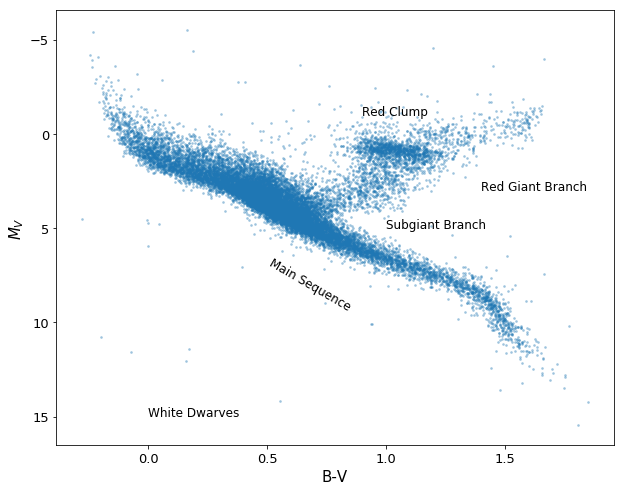
\includegraphics[width=5in]{hrdiagram.png}
\caption{HR diagram using Hipparcos data. Important features highlighted}
\end{figure}

\begin{lstlisting}[language=Python]
#prepare column names for data tables
names=['Mass','Mbol', 'log Teff', 'log g', 'M(B)', 'M(V)',
       'M(R)', 'M(I)', 'B-V', 'B-R', 'B-I', 'V-R','V-I']
       
#read in the isochrone data. 
iso_37_6gyr = pd.read_table('snewz04bvri.iso',
	skiprows = np.arange(259,1776), header=3, sep='\s+',
	names=names)
iso_37_7gyr = pd.read_table('snewz04bvri.iso',
	skiprows =  np.arange(515,1776), header=261, sep='\s+',
	names=names)
iso_37_8gyr = pd.read_table('snewz04bvri.iso',
	skiprows =  np.arange(769,1776), header=517 ,sep='\s+',
	names=names)
iso_37_9gyr = pd.read_table('snewz04bvri.iso',
	skiprows =  np.arange(1020,1776),
	header=771 ,sep='\s+', names=names)
iso_37_10gyr = pd.read_table('snewz04bvri.iso', 
	skiprows =  np.arange(1272,1776),
        header=1022 ,sep='\s+', names=names)
iso_37_11gyr = pd.read_table('snewz04bvri.iso',
	skiprows =  np.arange(1525,1776),
	header=1274 ,sep='\s+', names=names)
iso_37_12gyr = pd.read_table('snewz04bvri.iso',
	header=1527 ,sep='\s+', names=names)

#do this over for the other two files. 
#I won't inflict further source code on the reader
#you just want to use different var names and file names

#make the multiplot
fig=plt.figure(figsize=(14,8))

plt.subplots_adjust(wspace=.001)
cmap = plt.cm.get_cmap('YlOrRd')
c_space=np.linspace(.3,.8,7)

ax1 = fig.add_subplot(131)
ax1.scatter(clean_hip['B-V'].data, clean_hip['MV'],
	alpha=.3, s=3, label=None)
ax1.plot(iso_37_6gyr['B-V'].astype('float'),
	 iso_37_6gyr['M(V)'].astype('float'),
	c=cmap(c_space[0]), label='6Gyr')
ax1.plot(iso_37_7gyr['B-V'].astype('float'),
	 iso_37_7gyr['M(V)'].astype('float'),
	c=cmap(c_space[1]), label='7Gyr')
ax1.plot(iso_37_8gyr['B-V'].astype('float'),
	 iso_37_8gyr['M(V)'].astype('float'),
	c=cmap(c_space[2]), label='8Gyr')
ax1.plot(iso_37_9gyr['B-V'].astype('float'), 
	iso_37_9gyr['M(V)'].astype('float'), 
	c=cmap(c_space[3]), label='9Gyr')
ax1.plot(iso_37_10gyr['B-V'].astype('float'), 
	iso_37_10gyr['M(V)'].astype('float'),
	c=cmap(c_space[4]), label='10Gyr')
ax1.plot(iso_37_11gyr['B-V'].astype('float'), 
	iso_37_11gyr['M(V)'].astype('float'), 
	c=cmap(c_space[5]), label='11Gyr')
ax1.plot(iso_37_12gyr['B-V'].astype('float'), 
	iso_37_12gyr['M(V)'].astype('float'), 
	c=cmap(c_space[6]), label='12Gyr')
ax1.text(1, -5, '[Fe/H] = +.37', fontsize=13 )
ax1.invert_yaxis()
ax1.set_ylabel('$M_{V}$', fontsize=15)
ax1.tick_params(axis='both', which='major', labelsize=13)
ax1.legend(loc='lower left')

#do this over for the other data.
#you just want to make sure you do
#ax2 = fig.add_subplot(132) and make the same plots on ax2
#same goes for ax3
\end{lstlisting}

\begin{figure}
\centering
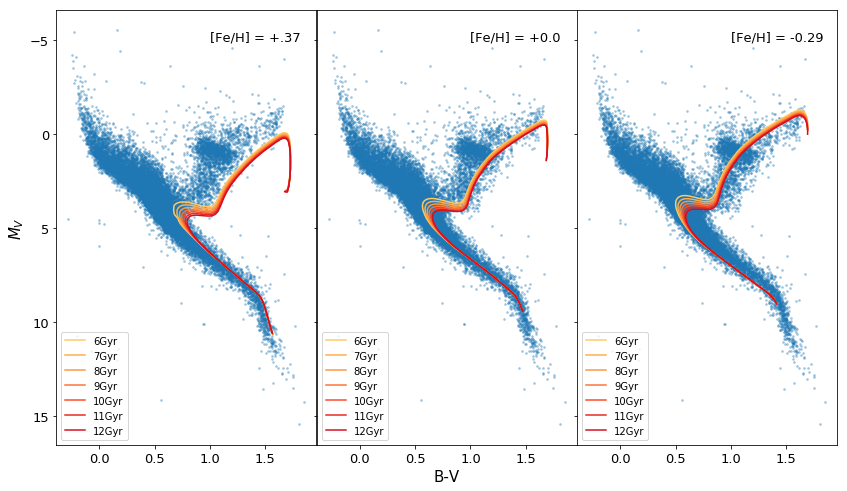
\includegraphics[width=6in]{isochrones.png}
\caption{isochrones for different metallicities overlaid the Hipparcos HR diagram}
\end{figure}

The isochrones for a metallicity of +.37 just doesn't seem right. It only captures the redder stars in the main sequence, and really doesn't capture the subgiants and giants. The metallicity 0.0 plot does a nice job of capturing the main sequence, even getting down to the M dwarves. On the other hand, only the younger stars are well fit in the sub giant and giant branch. The opposite is true with metallicity -0.29-the main sequence is not well fit (except for maybe the bluer part) but the giants and sub giants are well fit. If I had to choose, I would say the solar neighborhood has got metallicity 0.0 with 6Gyr old stars.

After reading the paper, I can see I made an overly simplified interpretation. I should have considered some linear combination of the models to explain different populations in the HR diagram. the lower envelop can be explained by the more metal rich stars, upper envelop by the metal poor stars, and middle ones by the metalicity 0.0 stars. 

\begin{figure}
\centering
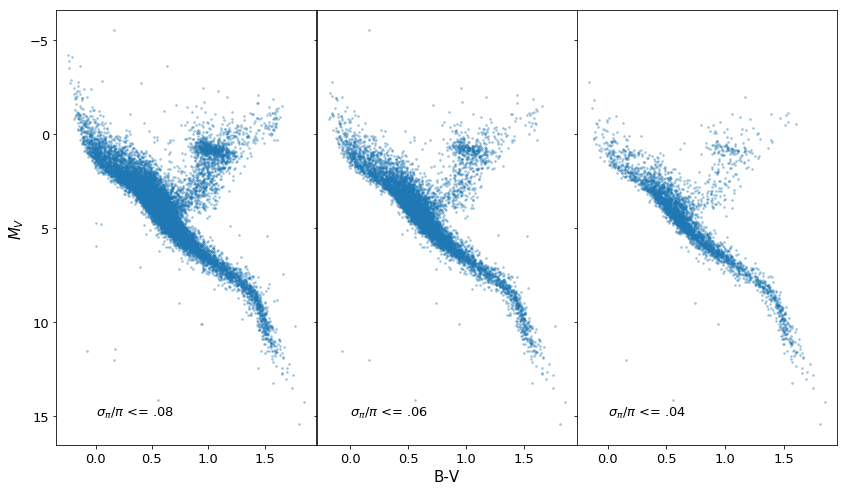
\includegraphics[width=6in]{hrpannels.png}
\caption{Hipparcos HR diagrams using different fractional uncertainty cuts in paralax}
\end{figure}

\end{document}